\chapter{Geometriske Algoritmer: Introduktion}

Geometriske Algoritmer (engelsk Computational Geometry) som studieområde kom frem i 1970'erne, hvor der blev studeret geometriske problemer, såsom at finde den hurtigste vej, given nogle forhindringer.

Vi definerer geometriske algoritmer som følger:

\begin{definition}[Geometriske Algoritmer]
	Den systematiske undersøgelse af algoritmer og datastrukturer for geometriske objekter, med et fokus på eksakte algoritmer som er asymptotisk hurtige.
\end{definition}

Hvert kapitel i bogen (Berg, Mark de) motiveres af et virkeligt beregningsproblem  som kræver geometriske algoritmer til sin løsning. Bogen forsøger at vise mange forskellige områder hvori geometriske algoritmer er brugbare, såsom robotteknologi,  computergrafik og geografisk informationsystemer.

\section{Konveks Skrog}%
\label{sec:label}

\index{konveks!definition}
\begin{definition}[Konveks]
	En delmængde $S$ af planen\footnote{En geometrisk plan} er \textit{konveks} hvis og kun hvis, for hvert par of punkter $p, q \in S$ er linjen der går fra $p$ til $q$ (eller omvendt) $\overline{pq}$ er komplet indeholdt i $S$.
\end{definition}

\begin{figure}
	\centering
	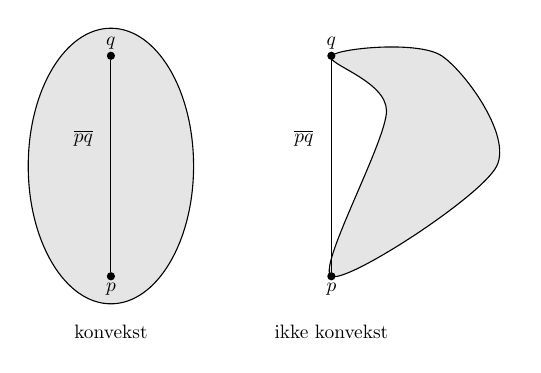
\begin{tikzpicture}[scale=0.7, transform shape]

		% Convex shape
		\begin{scope}
			\draw[fill=gray!20] (0,0) ellipse (1.5 and 2.5);
			\node[fill=black,circle,inner sep=1.5pt] (p1) at (0,-2) {};
			\node[fill=black,circle,inner sep=1.5pt] (q1) at (0,2) {};
			\draw (p1) -- (q1);
			\node[below] at (p1) {$p$};
			\node[above] at (q1) {$q$};
			\node at (-0.5,0.5) {$\overline{pq}$};
			\node at (0,-3) {konvekst};
		\end{scope}

		% Non-convex shape
		\begin{scope}[xshift=4cm]
			\draw[fill=gray!20] plot [smooth cycle] coordinates {(0,2) (2,2) (3,0) (0,-2) (1, 1) };
			\node[fill=black,circle,inner sep=1.5pt] (p2) at (0,-2) {};
			\node[fill=black,circle,inner sep=1.5pt] (q2) at (0,2) {};
			\draw (p2) -- (q2);
			\node[below] at (p2) {$p$};
			\node[above] at (q2) {$q$};
			\node at (-0.5,0.5) {$\overline{pq}$};
			\node at (0,-3) {ikke konvekst};
		\end{scope}

	\end{tikzpicture}
	\caption{\label{fig:konvekstornot} Eksempel på en linje der er konveks, og en der ikek er.}
\end{figure}

Man kan i figur~\ref{fig:konvekstornot} se to linjesegementer. Linjen til venstre i tegningen er konveks, da linjen forbliver på planen, hvor linjen til højre \textit{ikke} er konveks, da den går udaf planen.

\index{konveks!skrog!definition}
\begin{definition}[Konveks Skrog]
	Det \textit{konvekse skrog} (\textit{convex hull} på engelsk), skrevet $\mathcal{CH}(S)$ af en mængde $S$, er den \textit{mindste} konvekse mængde som indeholder $S$. Mere præcist er det fællesmængden af alle konvekse mængder som indeholder $S$.
\end{definition}

Bogen giver en visuel forklaring på et visuelt skrog. Kig på hvert punkt (knude) som var det et søm i en træbræt. Hvis du tager en elastik og holder den rundt om disse søm, når du giver slip vil du have et minimums konveks skrog, da elastikken ikke vil tage overflødige søm med.


Vi vil nu kigge på problemet om at beregne det konvekse skrog af en endelig mængde $P$ af $n$ punkter på planen. Vi får fra den tidligere visuelle beskrivelse en alternativ definition af konveks skrog:

\index{konveks!skrog!definition!alternativ}
\begin{definition}[Konveks Skrog]
	Et konvekst skrog er en unik konveks polygen hvis knuder er punkter fra mængden $P$ som indeholder alle punkter af $P$.
\end{definition}

Vi har tidligere sagt at vi vil løse problemet om beregning af en konveks skrog. Vi specificerer nu: Givet en mængde $P = \{p_{1}, p_{2}, \ldots, p_{n}\}$ af punkter på planen, udregn en liste som indeholder disse punkter fra $P$ som er knuder af $\mathcal{CH}(P)$, arrangeret i en orden der går \textit{med uret}.

Vores observation at $\mathcal{CH}(P)$ er en konveks polygen er brugbar til løsningen af problemet. Hvis vi tager en linje mellem to punkter $p$ og $q$, og alle punkter ligger til højre for linjen $\overline{pq}$, så må $\overline{pq}$ være en kant i den konvekse polygon.

\begin{algorithm}
	\caption{\label{alg:slowconvexhull}LangsomKonveksSkrog(P)}
	\begin{algorithmic}[1]
		\STATE E $\gets \emptyset$
		\FOR{alle ordnet par $(p,q) \in P \times P$ hvor $p \ne q$}
		\STATE \textit{valid} $\gets$ \textbf{true}
		\FOR{alle punkter $r \in P$ hvor $r \ne p$ og $r \ne q$}
		\IF{$r$ ligger til venstre for linjen fra $p$ til $q$}
		\STATE \textit{valid} $\gets$ \textbf{false}.
		\ENDIF
		\ENDFOR
		\IF{\textit{valid}}
		\STATE Tilføj den rettet kant $\stackrel{\rightarrow}{pq}$ til $E$.
		\ENDIF
		\ENDFOR
		\STATE Fra mængden $E$ af kanter, konstruér en liste $\mathcal{L}$ fra knuderne af $\mathcal{CH}(P)$ sorteret med klokken.
	\end{algorithmic}
\end{algorithm}


%%% Local Variables:
%%% mode: latex
%%% TeX-engine: luatex
%%% TeX-command-extra-options: "-shell-escape"
%%% TeX-master: "main"
%%% End:
